\chapter{Particle Identification}

% -----------------------------------------
%    chapter motivation and purpose 
% -----------------------------------------

\section{Introduction}
Particle identification (PID) is the process of classifying tracks as known particles.  After reconstruction and matching of detector responces to each track, the reconstruction package \texttt{recsis} assigns a preliminary particle identification based on loose selection criteria.  In this analysis, tracks are classified based on a more stringent criteria.  This chapter discusses the methodology used by the authors to classify particles.

\section{Electron Identification}
Electrons in CLAS are abundant, and the detection of an electron is a basic necessity for every event that will be analyzed.  Each negative track is considered a possible electron, a series of physically motivated cuts is applied.  If a track passes all cuts, it is identified as an electron.  All track indices which pass electron identification are saved, and the one with the highest momentum is used in the analysis.  
\\


\subsection{Electron ID Cuts}

The cuts used to select electrons are enumerated below.

\begin{itemize}
  \item{Negative charge}
  \item{Drift chamber region 1 fiducial}
  \item{Drift chamber region 3 fiducial}
  \item{Electromagnetic Calorimeter fiducial (UVW)}
  \item{EC minimum energy deposition}
  \item{Sampling Fraction (momentum dependent)}
  \item{z-vertex position}
  \item{Cherenkov counter $\theta_{cc}$ matching to PMT number}
  \item{Cherenkov counter $\phi_{rel}$ matching to PMT (left/right)}
\end{itemize}

Each cut will now be described in more detail.

\subsubsection*{Negativity Cut}
Each track is assigned a charge based on the curvature of it's trajectory through the magnetic field of the torus.  This is done during the track reconstruction phase.  The tracks are eliminated as electron candidates if they are not negatively charged.

\subsubsection*{Drift chamber fiducial}
Negative tracks which pass geometrically close to the edges of the drift chamber are, from a tracking perspective, more difficult to understand.  Often these tracks originate from downstream background, or are otherwise unacceptable.  Additionally, tracks which fall outside of the fiducial region of the drift chambers are likely to fall outside of the fiducial region of the downstream detectors as well.  For these reasons, it is common to remove tracks which are geometrically close to the boundaries of the drift chambers in region 1 as well as region 3 coordinate systems.

\subsubsection*{Electromagnetic Calorimeter fiducial (UVW)}
As tracks traverse the electromagnetic calorimeter they develop electromagnetic showers.  If the track passes close to the edges of the detector, there is a chance that the shower will not be fully contained within the calorimeter volume (it spills out the edges).  For this reason, it has become standard to remove the hits which fall within the outer 10 centimeters of each layer of the EC (10 centimieters is the width of a scintillator bar).  This cut is applied in the U, V, W coordinate system.  

\begin{table}
  \centering
  \begin{tabular}{c|c|c}
    EC Coordinate & Min (cm) & Max (cm) \\
    U & 70 & 400 \\
    V & - & 362 \\
    W & - & 395
  \end{tbular}
  \caption{Cut parameters used for the EC fiducial cut.}
\end{table}

\easyFigure{image/plots/electron-id/ec-fid.png}{All negative tracks are shown here in black.  In color, the tracks which pass the EC fiducial cut are shown.}

\subsubsection*{EC minimum energy deposition}
The negative tracks that start out as electron candidates are primarily composed of electrons and negative $\pi$ mesons.  One way to differentiate between these two species is to exploit the difference in energy deposition between the two in the electromagnetic calorimeter.  Electron typically develop a much larger more energetic shower than $\pi$ mesons, which minimally ionize the calorimeter material.  The result is that the total energy deposition is typically larger for electrons than $\pi$ mesons.  In this analysis we require that at least 60 MeV was deposited in the inner calorimeter for electron candidates.  

\subsubsection*{Sampling Fraction (momentum dependent)}
The electromagnetic calorimeter is designed such that electrons will deposit $E_{dep}/p \approx 0.3$ approximately one-third of their energy, regardless of their momentum.  In contrast to this, the ratio $E_{dep}/p$ for $\pi$ mesons decreases rapidly with momentum.  To develop a momentum dependent cut for this distribution, all negative candidates are first filled into a two-dimensional histogram of $E_{dep}/p$ vs. $p$.  The histogram is then binned more coarsely in momentum, and projected into a series of 40 slices.  Each of these slices is fit with a Gaussian to extract the position $\mu_i$ and width $\sigma_i$ of the electron peak.  Finally, the authors choose a functional form for the mean and standard deviation of the distributions to be a third order polynomial in momentum.

\begin{eqnarray}
  \mu (p) = \mu_0 + \mu_1 p + \mu_2 p^2 + \mu_3 p^3 \\
  \sigma (p) = \sigma_0 + \sigma_1 p + \sigma_2 p^2 + \sigma_3 p^3 
\end{eqnarray}    

Boundaries are constructed from this information by adding/subtracting $n_{\sigma}$ from the mean.  In the nominal case, we use $n_{\sigma} = 2.5$.

\begin{eqnarray}
  f_{max} (p) = \mu (p) + n_{\sigma} \sigma (p) = (\mu_0 + n_{\sigma} \sigma_0) + (\mu_1 + n_{\sigma} \sigma_1)p + (\mu_2 + n_{\sigma} \sigma_2)p^2 + (\mu_3 + n_{\sigma} \sigma_3)p^3 \\
  f_{min} (p) = \mu (p) - n_{\sigma} \sigma (p) = (\mu_0 - n_{\sigma} \sigma_0) + (\mu_1 - n_{\sigma} \sigma_1)p + (\mu_2 - n_{\sigma} \sigma_2)p^2 + (\mu_3 - n_{\sigma} \sigma_3)p^3
\end{eqnarray}

Due to slight differences between the 6 sectors of the CLAS detector, the authors choose to calibrate and apply this cut for each sector individually.  The results are shown in table \ref{table-sampling-fraction}.

% ---------------------------------
%  table of cut values for this 
% ---------------------------------

\begin{table}[h]
  \centering 

  \begin{tabular}{c | c | c | c | c | c | c}
    Parameter & Sector 1 & Sector 2 & Sector 3 & Sector 4 & Sector 5 & Sector 6                           \\
    \hline
    $\mu_3$     & -8.68739e-05 & 0.000459313  &  9.94077e-05 & -0.000244192 & -7.65218e-05 & -0.000392285  \\
    $\mu_2$     & -0.000338957 & -0.00621419  & -0.00267522  & -0.00103803  & -0.00222768  & -0.00105459   \\
    $\mu_1$     &  0.0191726   &  0.0393975   &  0.02881     &  0.0250629   &  0.0233171   &  0.0265662    \\
    $\mu_0$     &  0.2731      &  0.296993    &  0.285039    &  0.276795    &  0.266246    &  0.25919      \\
    $\sigma_3$  & -0.000737136 &  0.000189105 & -0.000472738 & -0.000553545 & -0.000646591 & -0.000633567  \\
    $\sigma_2$  &  0.00676769  & -0.000244009 &  0.00493599  &  0.00434321  &  0.00717978  &  0.00626044   \\
    $\sigma_1$  & -0.0219814   & -0.00681518  & -0.0180929   & -0.0140827   & -0.0246181   & -0.022029     \\
    $\sigma_0$  &  0.0474188   &  0.0475098   &  0.0461743   &  0.0492728   &  0.0546257   &  0.0517508    
  \end{tabular}
  \caption{$\mu$ and $\sigma$ values used to construct the momentum dependent sampling fraction cut.}
  \label{table-sampling-fraction}
\end{table}

\subsubsection*{z-vertex position}
Electrons can be produced as part of $e^+ e^-$ pairs.  For this analysis, these are not of interest.  The authors choose to select only electrons which originate from the target and are believed to be the scattered incoming electron.  For this reason the authors accept only electron candidates which have a z-vertex $v_z \in [-27.7302, -22.6864]$.  This cut is applied after the vertex position has been corrected (this correction will be discussed in a subsuquent chapter).

\subsubsection*{Cherenkov counter $\theta_{cc}$ and $\phi_{rel}$ matching to PMT}
The placement of photo-multiplier tubes (PMT) in the Cherenkov counter allows for additional consistency conditions to be applied.  The placement of 18 PMTs increasing in polar angle away from the beamline means that the PMT segment number is correlated to the angle which the electron has with the beamline at the Cherenkov counter $\theta{cc}$.  Additionally, PMTs that are placed on the left and right of the detector can be used to check consistency with the azimuthal angle the track forms with the central line of the detector (ie $\phi_{rel} > 0$ means the track was in the right half of the sector, $\phi_{rel} < 0$ means the track was in the left half of the sector).  An integer code is used to describe the PMT associated with the track.  The left PMT is assigned value -1, the right 1, and a signal in both PMTs is assigned 0.  If both PMTs have a signal, the track is allowed to pass.  If the left PMT was the one that had a signal, only events with $\phi_{rel} < 0$ are allowed to pass.  Similarly if the right PMT fired (code = 1), only events with $\phi_{rel} > 0$ are allowed to pass.  Technical note: the integers in question can be obtained from the ntuple22 format tree by doing the following.

\begin{lstlisting}
  for (int index = 0; index < event.gpart; index++){
    int pmt = event.cc_segm[index]/1000 - 1;
    int segment = event.cc_segm[index]%1000/10; 
  }
\end{lstlisting}

\easyFigure{image/diagrams/relative-phi.pdf}{The angle $\phi_{rel}$ is the azimuthal angle between the central line of the detector and the track.}


\section{Hadron Identification}
First, electrons are identified and any additional (not electrons) tracks in the event are processed.  Second, cuts are applied to remove tracks in poorly understood regions of the detector.  An additional cut is used for our analyses which restricts the vertex of the track to be close to that of the electron.  Such a cut should be removed to study processes with detached vertex positions (arising from the decay of other produced hadrons). Next, the species of particle is chosen based on the likelihood ratio.  Finally, a minimum confidence level for each track is required.  \\

The likelihood methodology described in this section is based on the discussion provided by the BES collaboration \cite{bes_physics}.  

\subsection*{Preliminary Cuts}

% ----------------------------------------------
%        cuts used before likelihood 
% ----------------------------------------------

After electron identification, all remaining tracks are subject to two constraints.  First, events which pass close to the torus coils are removed by cutting on the hit positions reported by the region 1 drift chambers, this is shown in figure \ref{fig:fid}.  Such events are often poorly reconstructed or have poorly understood acceptances and are discarded from analyses.  Then, the distance between the electron vertex and the hadron candidate track vertex is computed ($\delta v_{z} = v_{z}^{e} - v_{z}^{+}$).  This distance is constrained to be within the length of the target (5 cm) see figure \ref{fig:dvz}.  As stated above, if the analyst desires to look at events where the hadron is produced as the result of a decaying hadron, this cut should be removed.  

\begin{figure}
  \label{fig:dvz}
  \begin{center}
    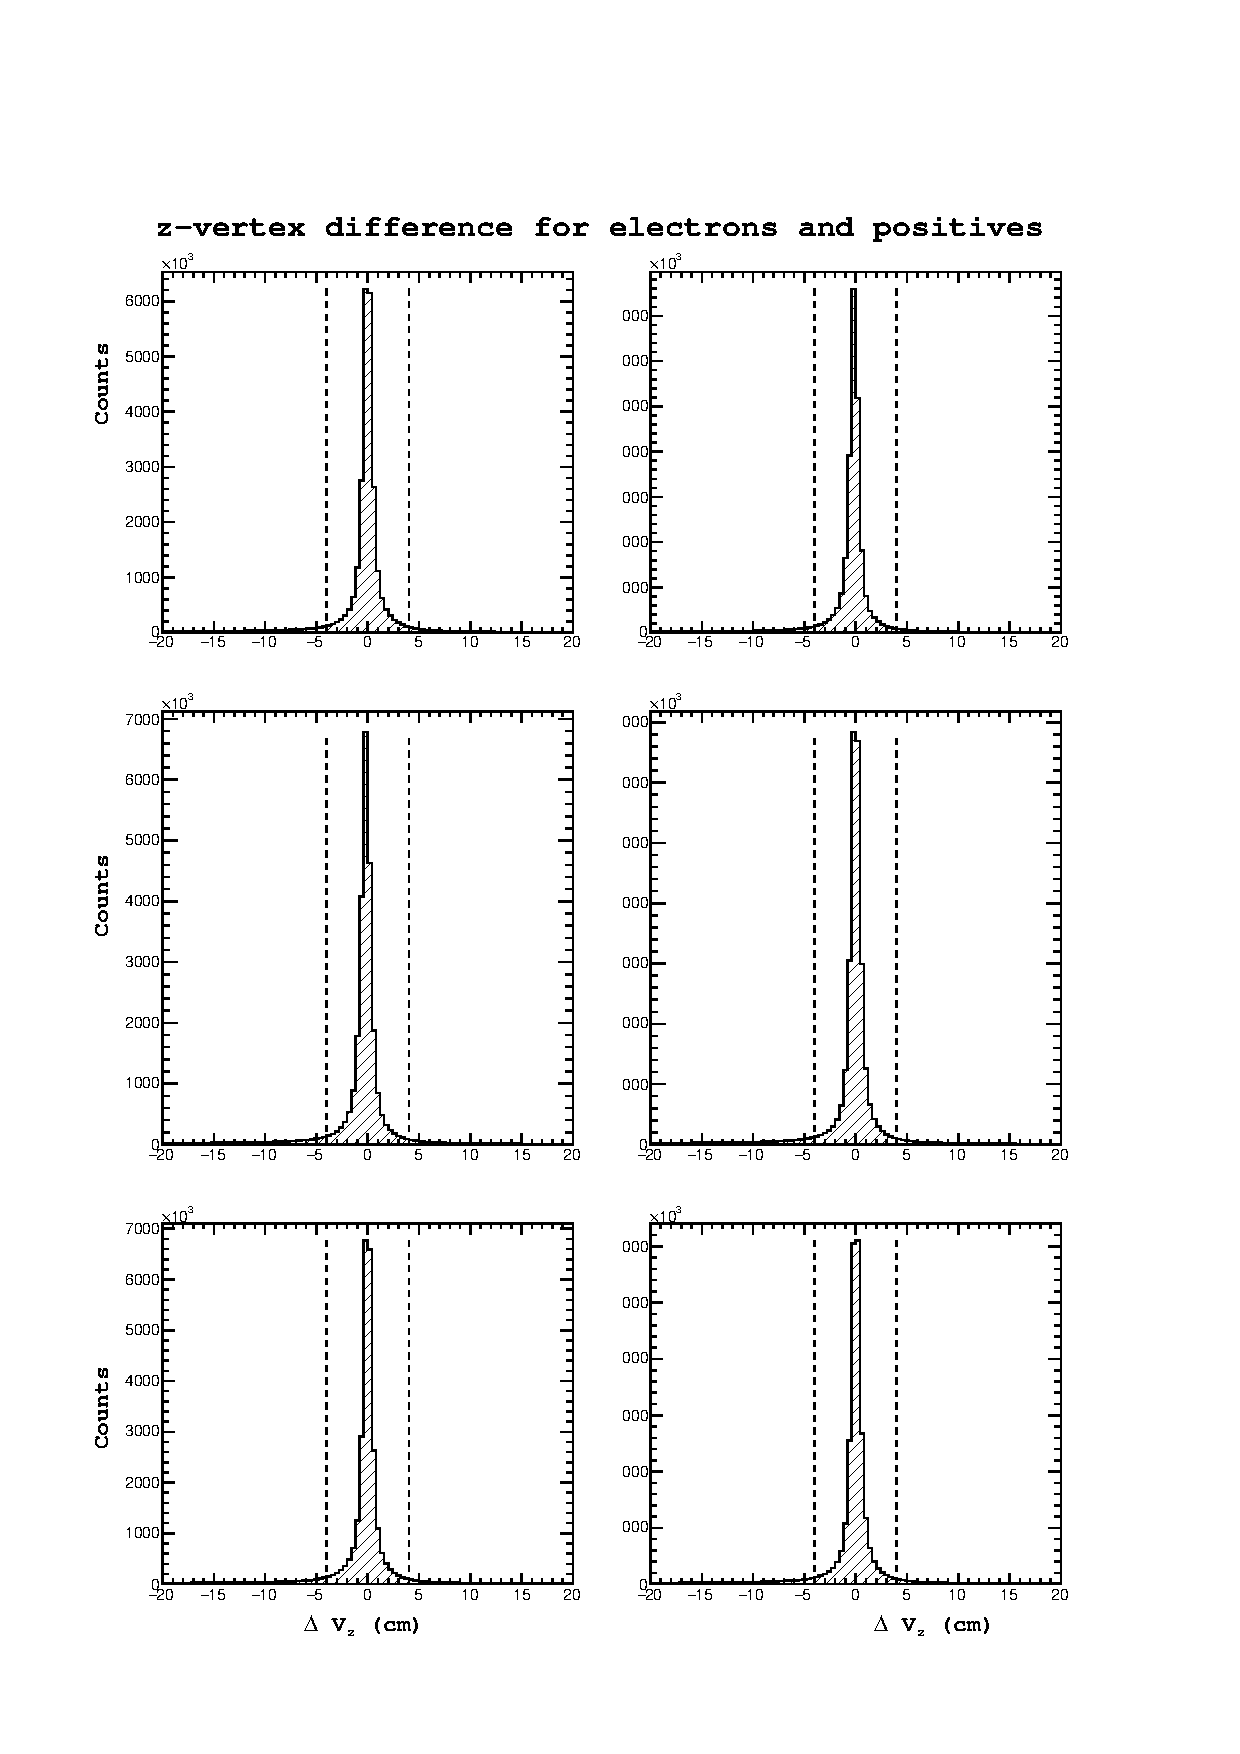
\includegraphics[width=10cm]{image/plots/hadron-id/dvz.pdf}
    \caption{Shown above: The difference between the z-vertex position between detected electrons and positive tracks.}
  \end{center}
\end{figure}

\begin{figure}
  \label{fig:fid}
  \begin{center}
    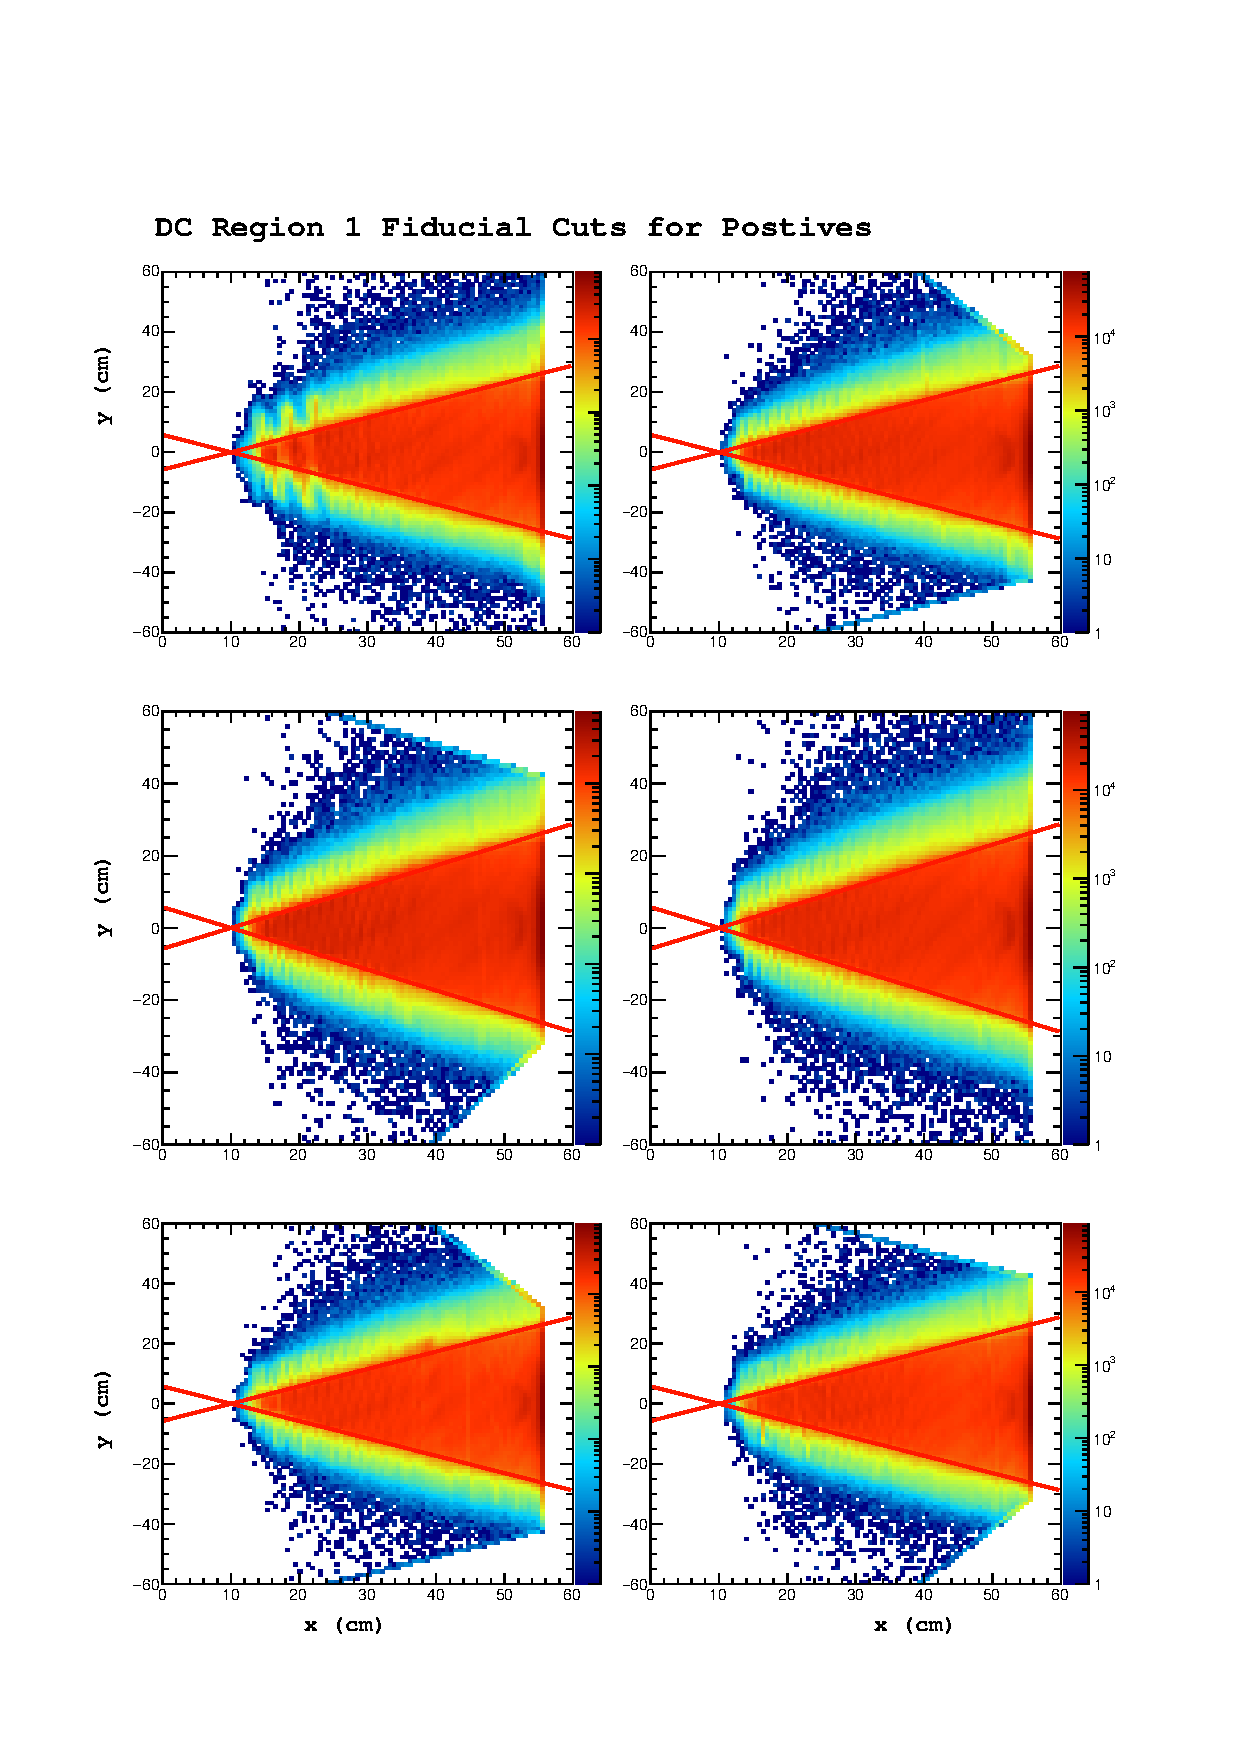
\includegraphics[width=10cm]{image/plots/hadron-id/fid.pdf}
    \caption{Shown above: Positive track hits on the region 1 drift chamber, events falling between the red lines are kept for analysis.}
  \end{center}
\end{figure}

%
% These really don't add anything to the discussion 
%
%\begin{figure}
%  \begin{center}
%    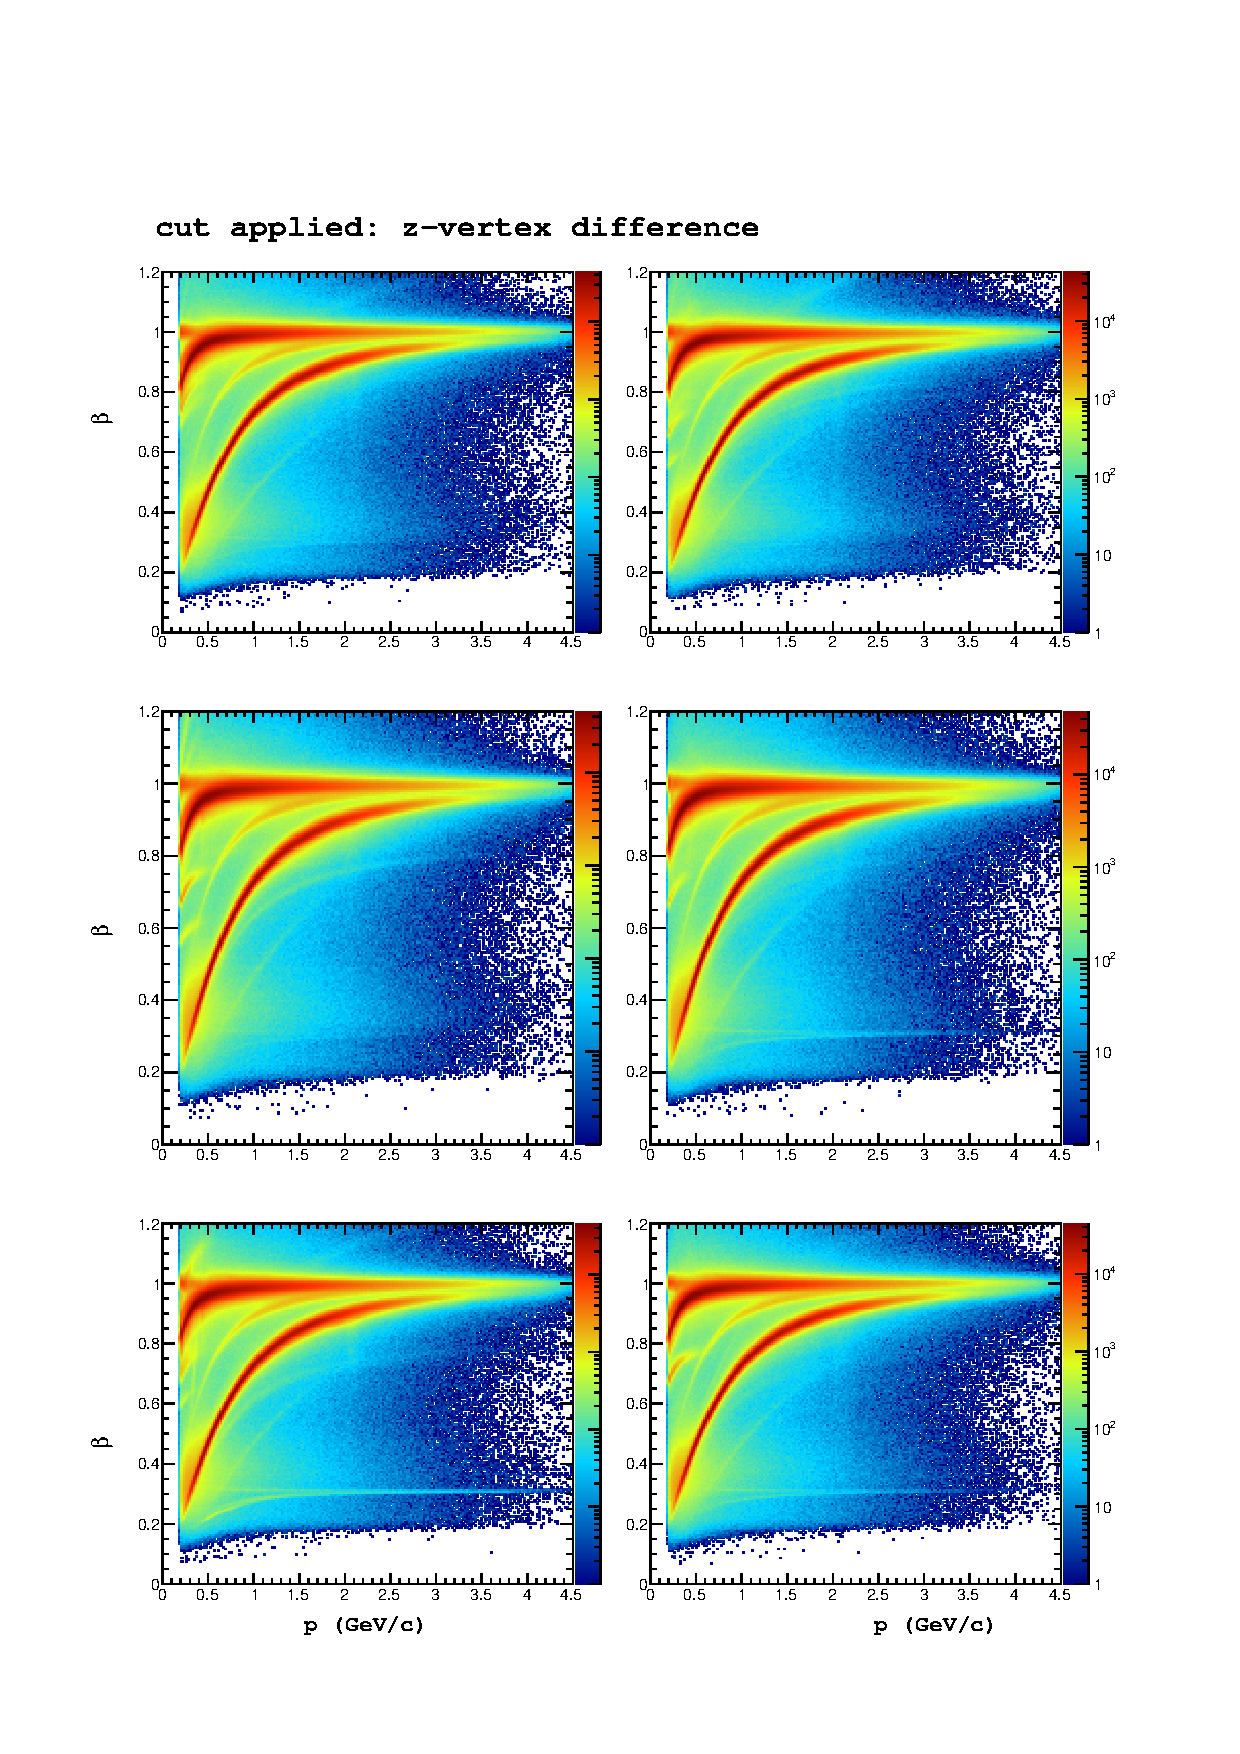
\includegraphics[width=10cm]{image/p_beta_dvz.pdf}
%    \caption{Shown above: }
%  \end{center}
%\end{figure}

%\begin{figure}
%  \begin{center}
%    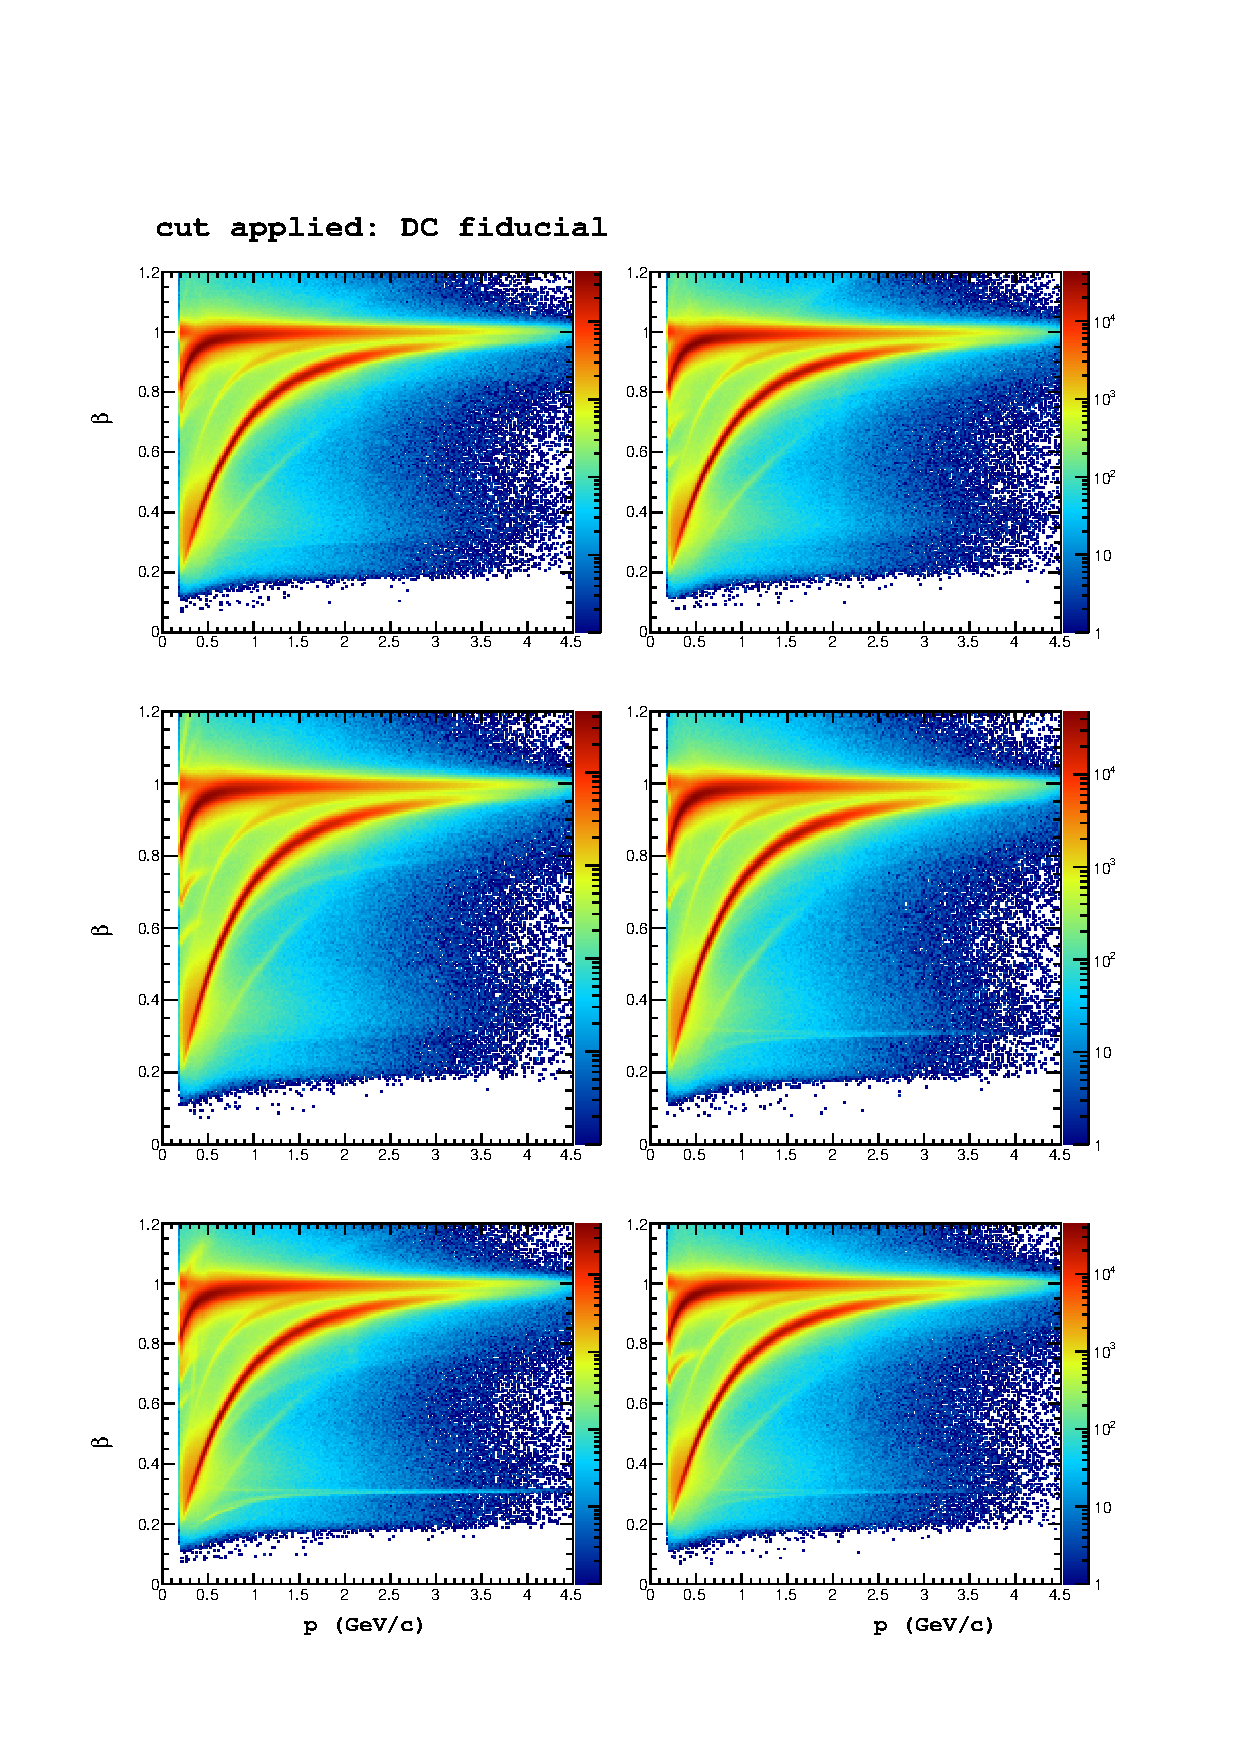
\includegraphics[width=10cm]{image/p_beta_fid.pdf}
%    \caption{Shown above: }
%  \end{center}
%\end{figure}

\subsection*{Likelihood Method}
In this section, positive hadrons are used as an example.  The same method is applied to the negative hadrons.  For each particle species considered, a normalized probability density function $P(x;p,h)$ is constructed for each input into the likelihood analysis.  Here, x corresponds to the feature being used to catagorize different particles (in our case, x is the $\beta$ value measured by CLAS time-of-flight), p is the particle momentum, and h is the hadron being hypothesized (eg: in our case the possible values for positive hadrons are pion, kaon, proton).  In general if one uses a set of $N$ variables $x = (x_1, x_2, ..., x_N)$, the likelihood for a hypothesis h is defined below.

\begin{equation}
  \mathcal{L}_h = \prod^{N}_{i=1} P_{i} (x_i; p, h)
\end{equation}

In our case, the only random variable we consider is $\beta$, and the likelihood is just the PDF.  Here, and in many cases where the choice is statistically appropriate, it is possible to use a Gaussian PDF for the variable $x_i$ ($\beta$).

\begin{equation}
  P(\beta;p,h) = \frac{1}{\sqrt{2 \pi} \sigma_\beta(p,h) } exp \left \{ -\frac{1}{2} \bigg( \frac{\beta - \mu_\beta(p,h)}{\sigma_\beta(p,h)} \bigg)^2 \right \}
\end{equation}

The identity is assigned by choosing the particle hypothesis h which maximizes the likelihood ratio.  
 
\begin{equation}
  \frac{\mathcal{L}_h}{\mathcal{L}_{\pi}+\mathcal{L}_{K}+\mathcal{L}_{p}}
\end{equation}

Using this method, every positive track is assigned a particle identification.  However, at times the likelihood value is quite small when compared with the maximum likelihood for that species.  This is the case for positrons which are classified by this method as positive pions, because they are the closest particle for which a hypothesis has been provided.  To avoid these situations, the confidence level $\alpha$ of each track is calculated and a cut is applied on the minimum confidence.  This cut can be easily varied to see how it changes the analysis result.

\begin{equation}
  \alpha = 1 - \int_{\mu-\beta_{obs}}^{\mu+\beta_{obs}} P(\beta;p,h) d\beta
\end{equation}

This quantity represents the probability to observe a value of $\beta$ as far from the mean as $\beta_{obs}$.  Confidence levels of 0 then correspond to tracks which are poorly identified as the class h.  In the case that the PDF is Gaussian, the standard 1, 2, and 3 sigma cuts on $\beta$ vs. $p$ can be understood simply as confidence levels of approximately 0.32 = 1-0.68, 0.05 = 1-0.95, and 0.01 = 1-0.99.

\begin{figure}
  \begin{center}
    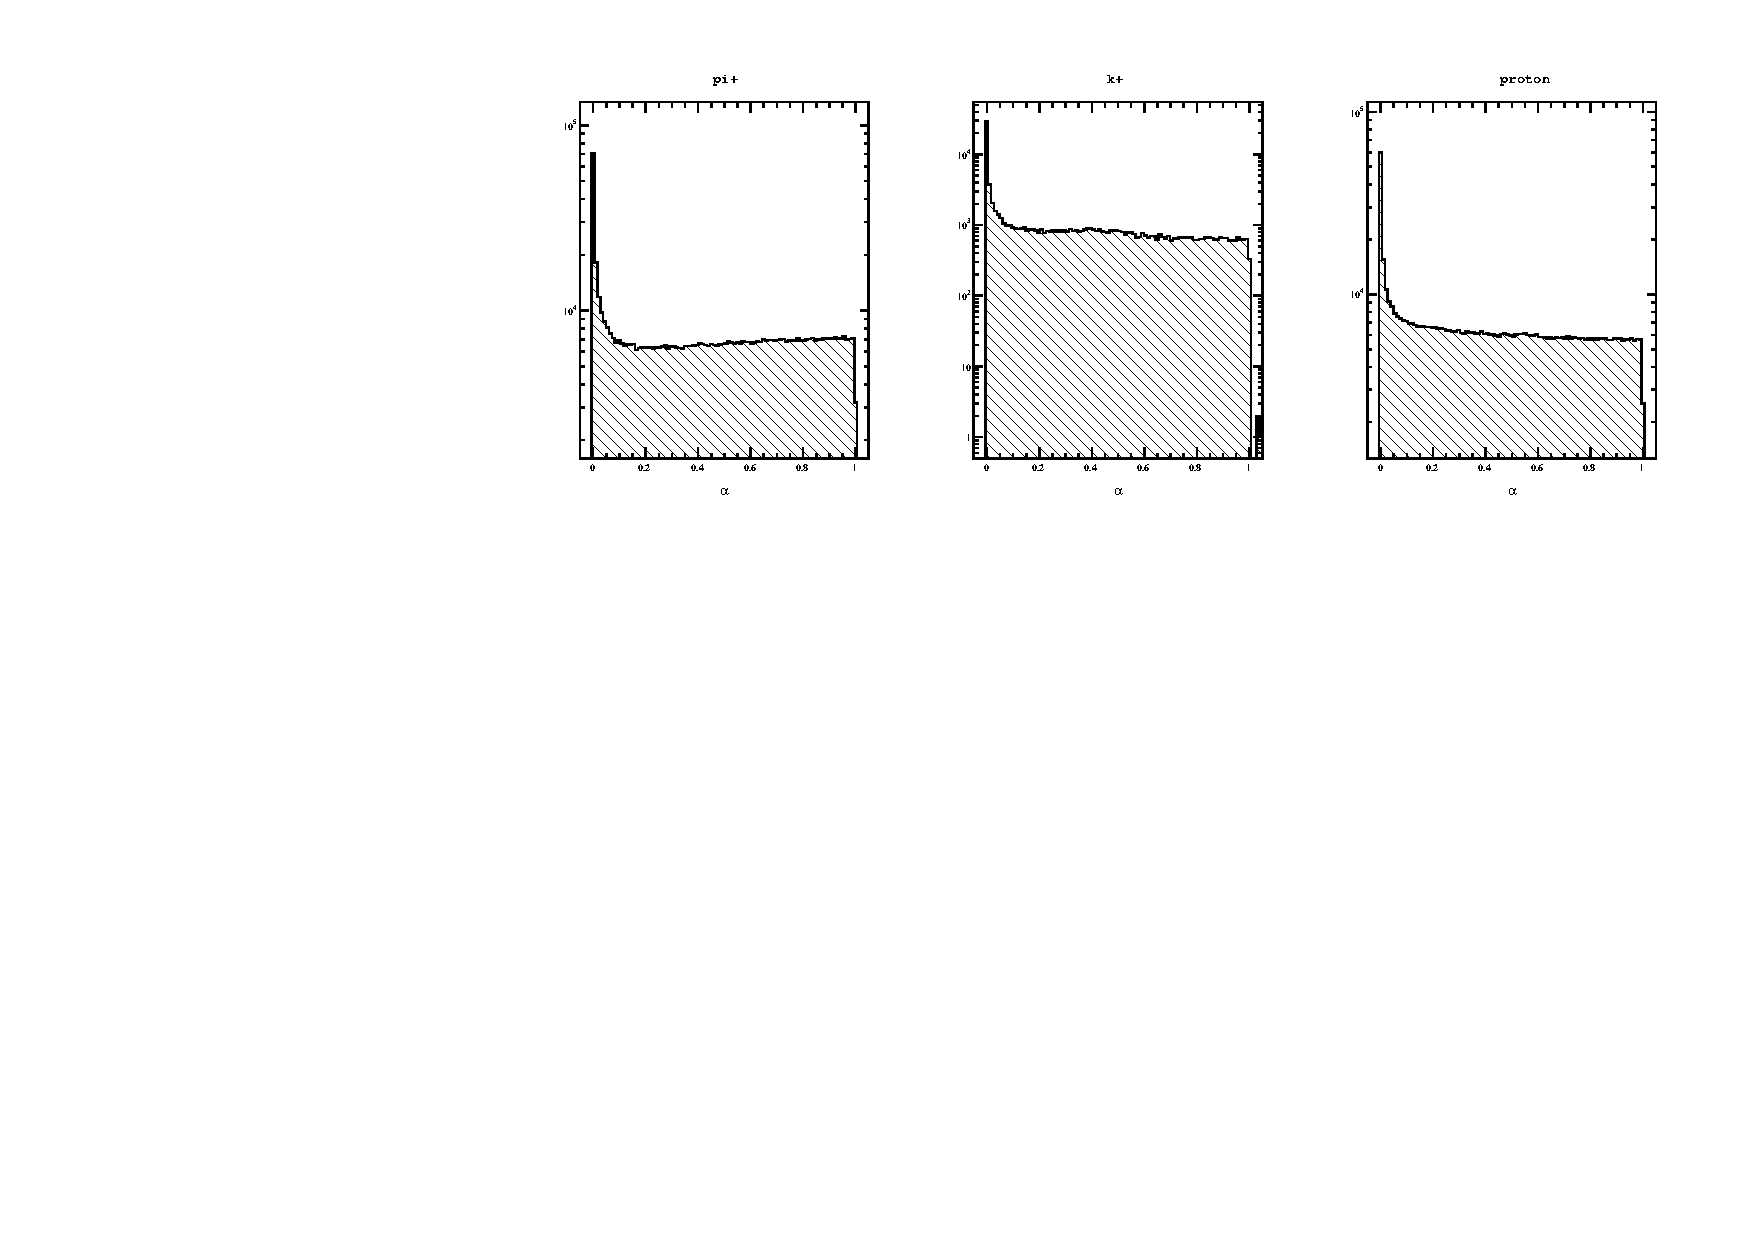
\includegraphics[width=14cm]{image/plots/hadron-id/confidence_level.pdf}
    \caption{ Shown above: The distribution of confidence level for all positive tracks after being classified by the likelihood ratio.}
  \end{center}
\end{figure}

\subsection*{Determination of Probability Density Functions}

The most important and most difficult part of constructing the likelihood ratio identification is the ascertation of the mean and standard deviation of the probability density function (which depends on momentum) for the different particle hypothesis.  In the case where exceptionally accurate monte carlo (MC) simulations of the detector are available, one can use the truth information and track matching to construct the $\beta$ vs. $p$ 2-dimensional histograms, and fit the $\mu(p)$ and $\sigma(p)$.  In the absence of high quality MC, analysts typically fit directly the spectrum of $\beta$ vs. $p$ and extract the mean and variance.  In this work, the authors chose to create an enhanced sample of candidates for each of the three positive particles in question before doing the fitting.  In this way, we hope to get a better quality fit of the true mean, and resolutions for the different species.  For fitting of pion and proton resolutions, positive tracks are assumed to be pions and the missing mass of the event is calculated.  Then, a cut is placed around the neutron mass.  In doing so, we are selecting mainly two types of exclusive events.  The first is $ep \rightarrow e\pi^+N$, and the second is $ep \rightarrow ep\pi^0$.  In this way most positrons, and positive kaons are removed from the sample prior to fitting.  The mean and variance are fit using a third order polynomial in p (MINUIT $\chi^2$ minimization is used).  The negative tracks $\pi^-$, $K^-$ are fit directly as is normally done.

\begin{figure}
  \begin{center}
    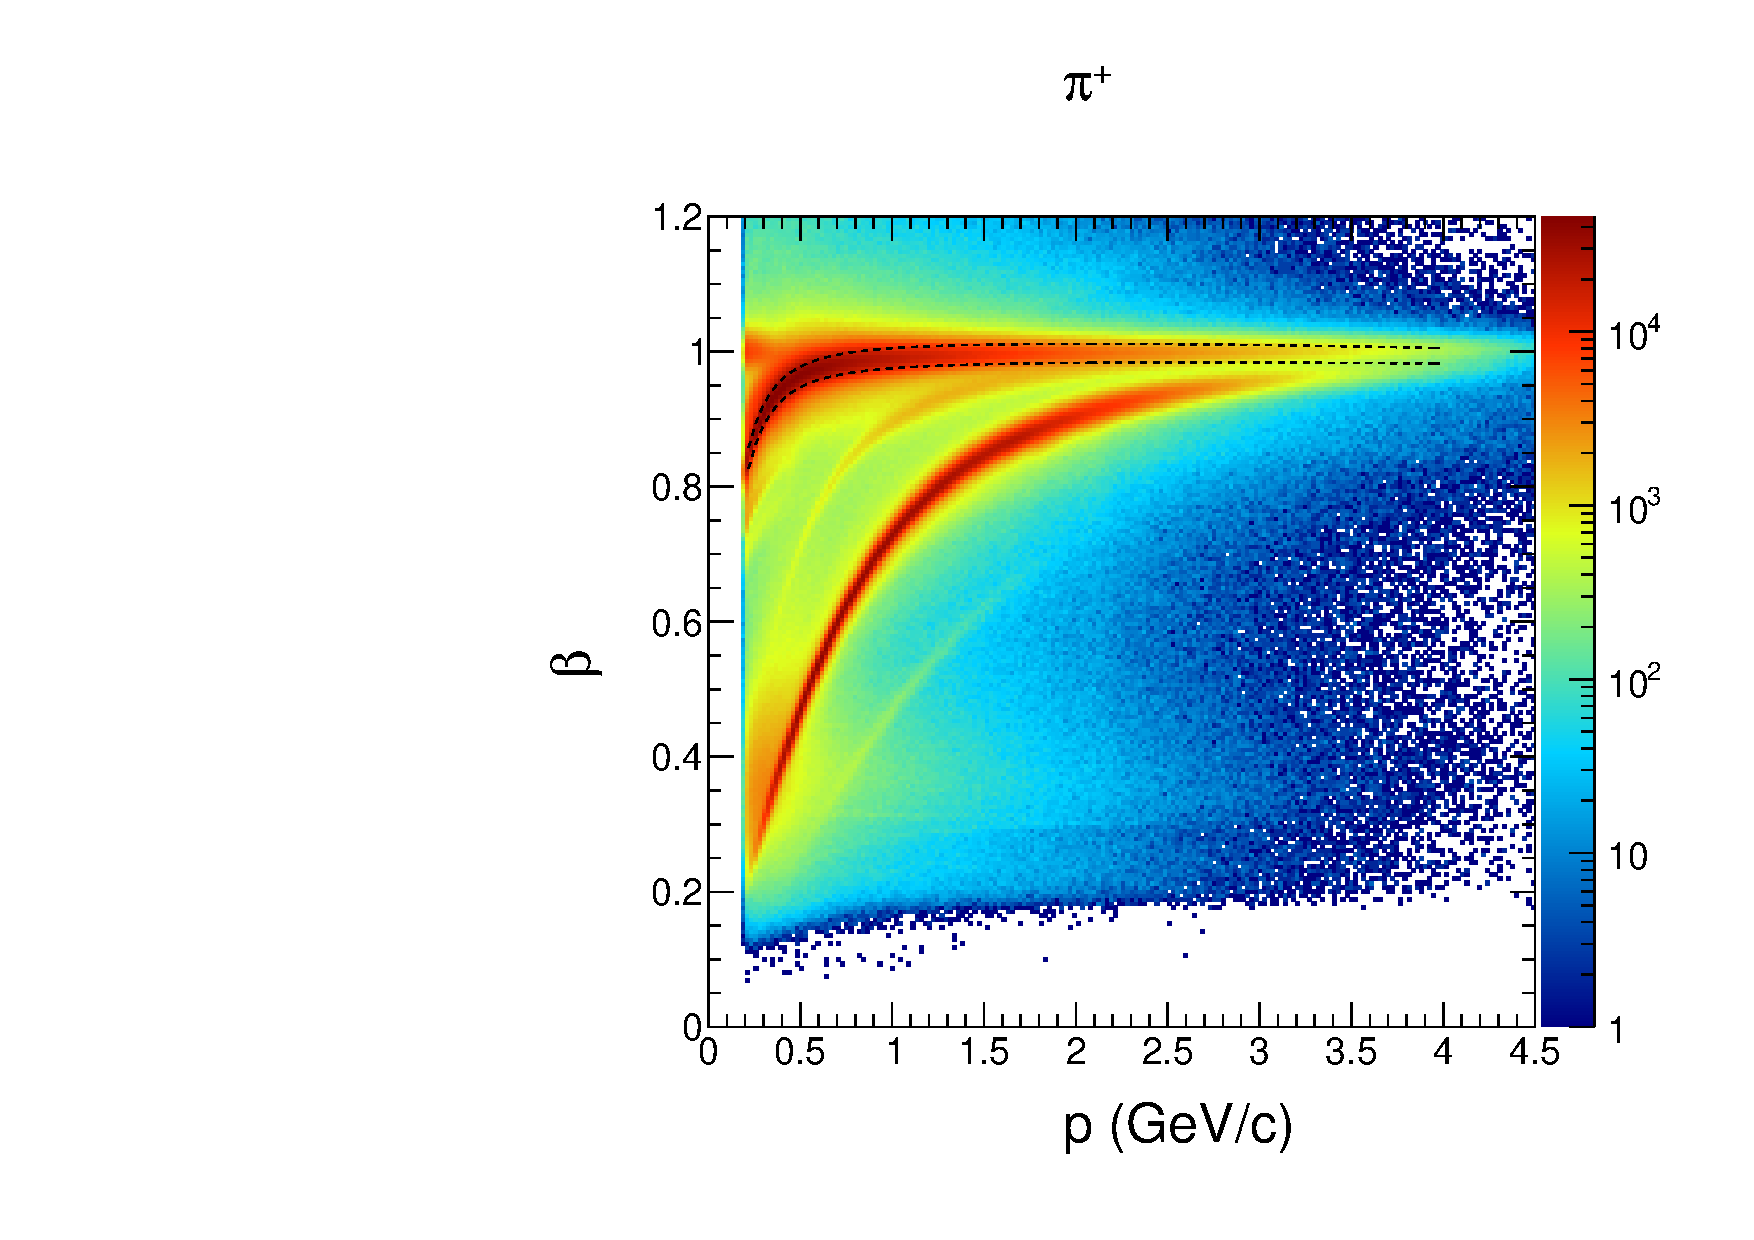
\includegraphics[width=10cm]{image/plots/hadron-id/beautiful_pbeta_pip.pdf}
    \caption{ Shown above: All positive tracks overlaid with our determination of $\mu(p) \pm \sigma(p)$ for $\pi^+$}
  \end{center}
\end{figure}

\begin{figure}
  \begin{center}
    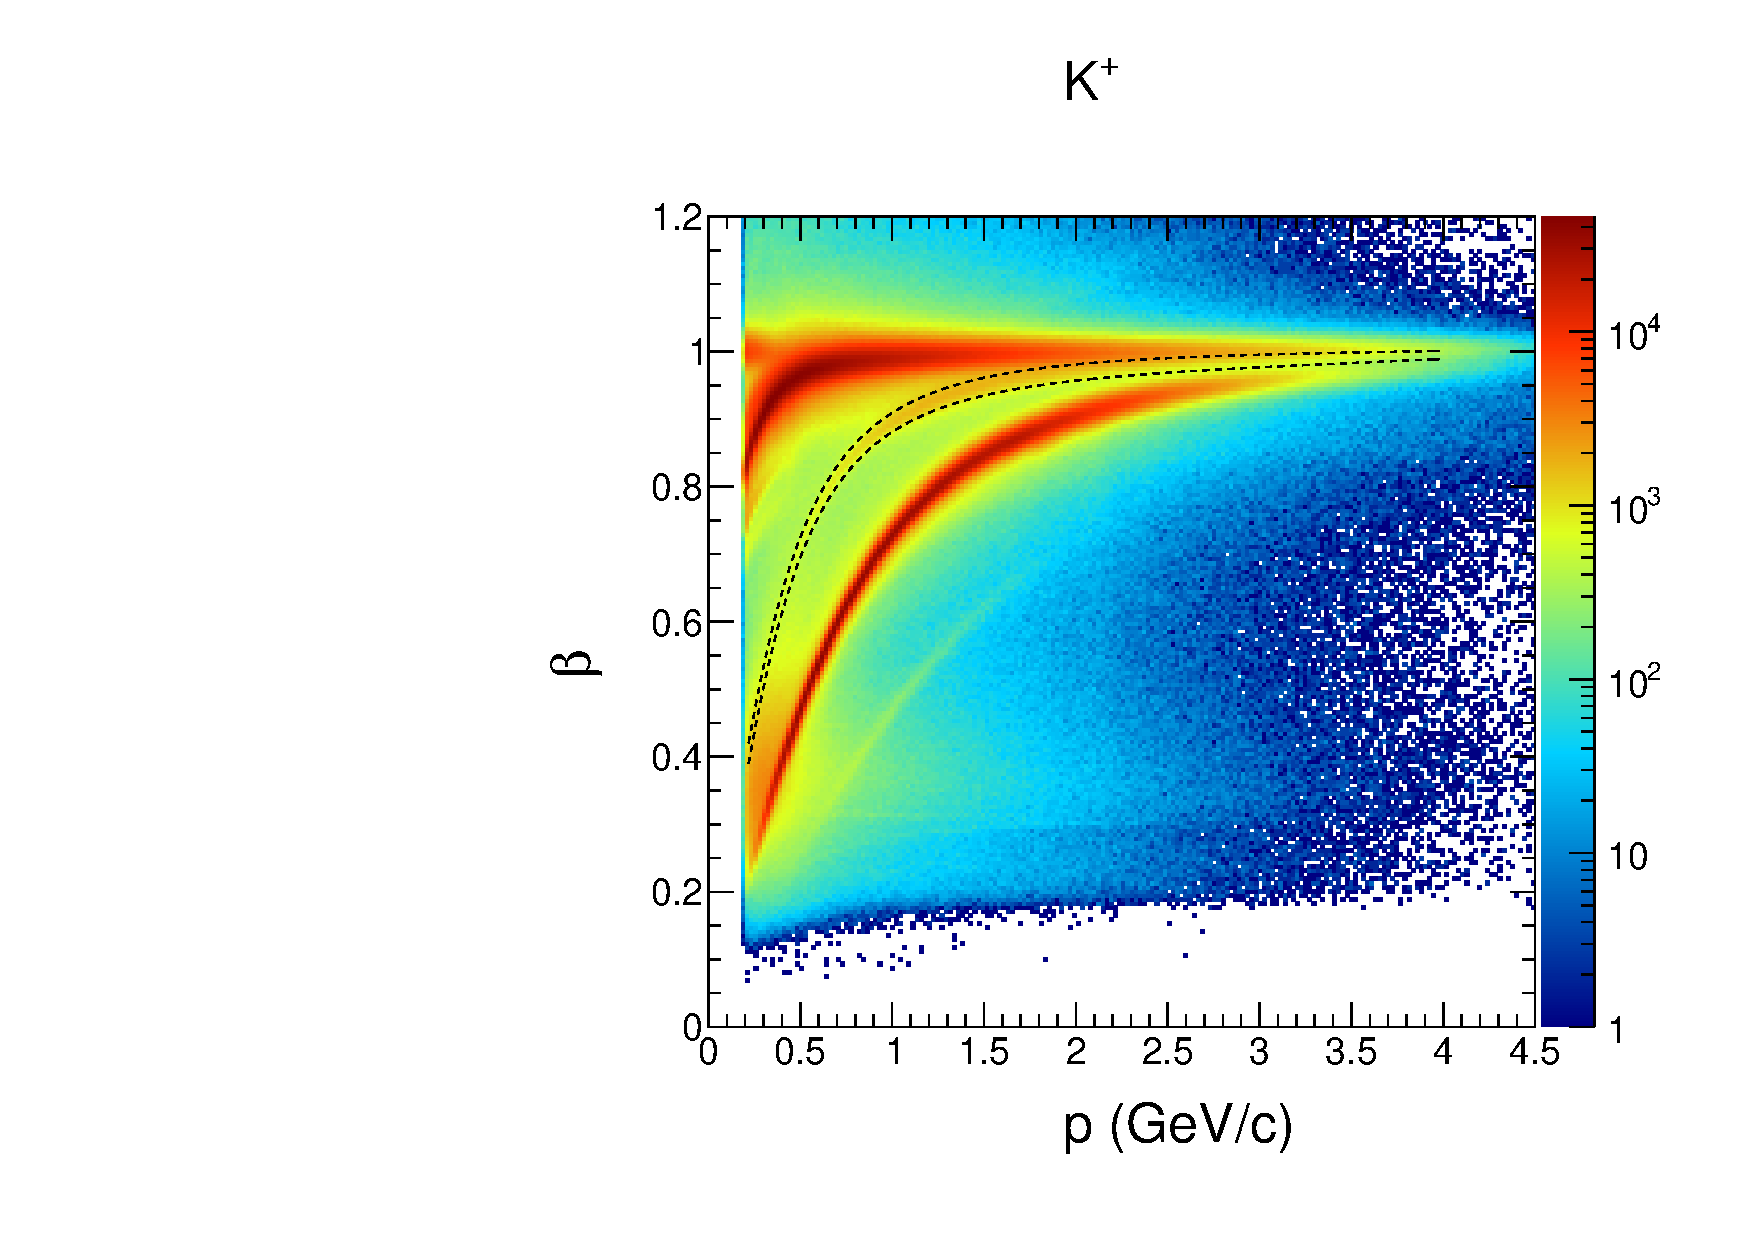
\includegraphics[width=10cm]{image/plots/hadron-id/beautiful_pbeta_kp.pdf}
    \caption{ Shown above: All positive tracks overlaid with our determination of $\mu(p) \pm \sigma(p)$ for $K^+$}
  \end{center}
\end{figure}

\begin{figure}
  \begin{center}
    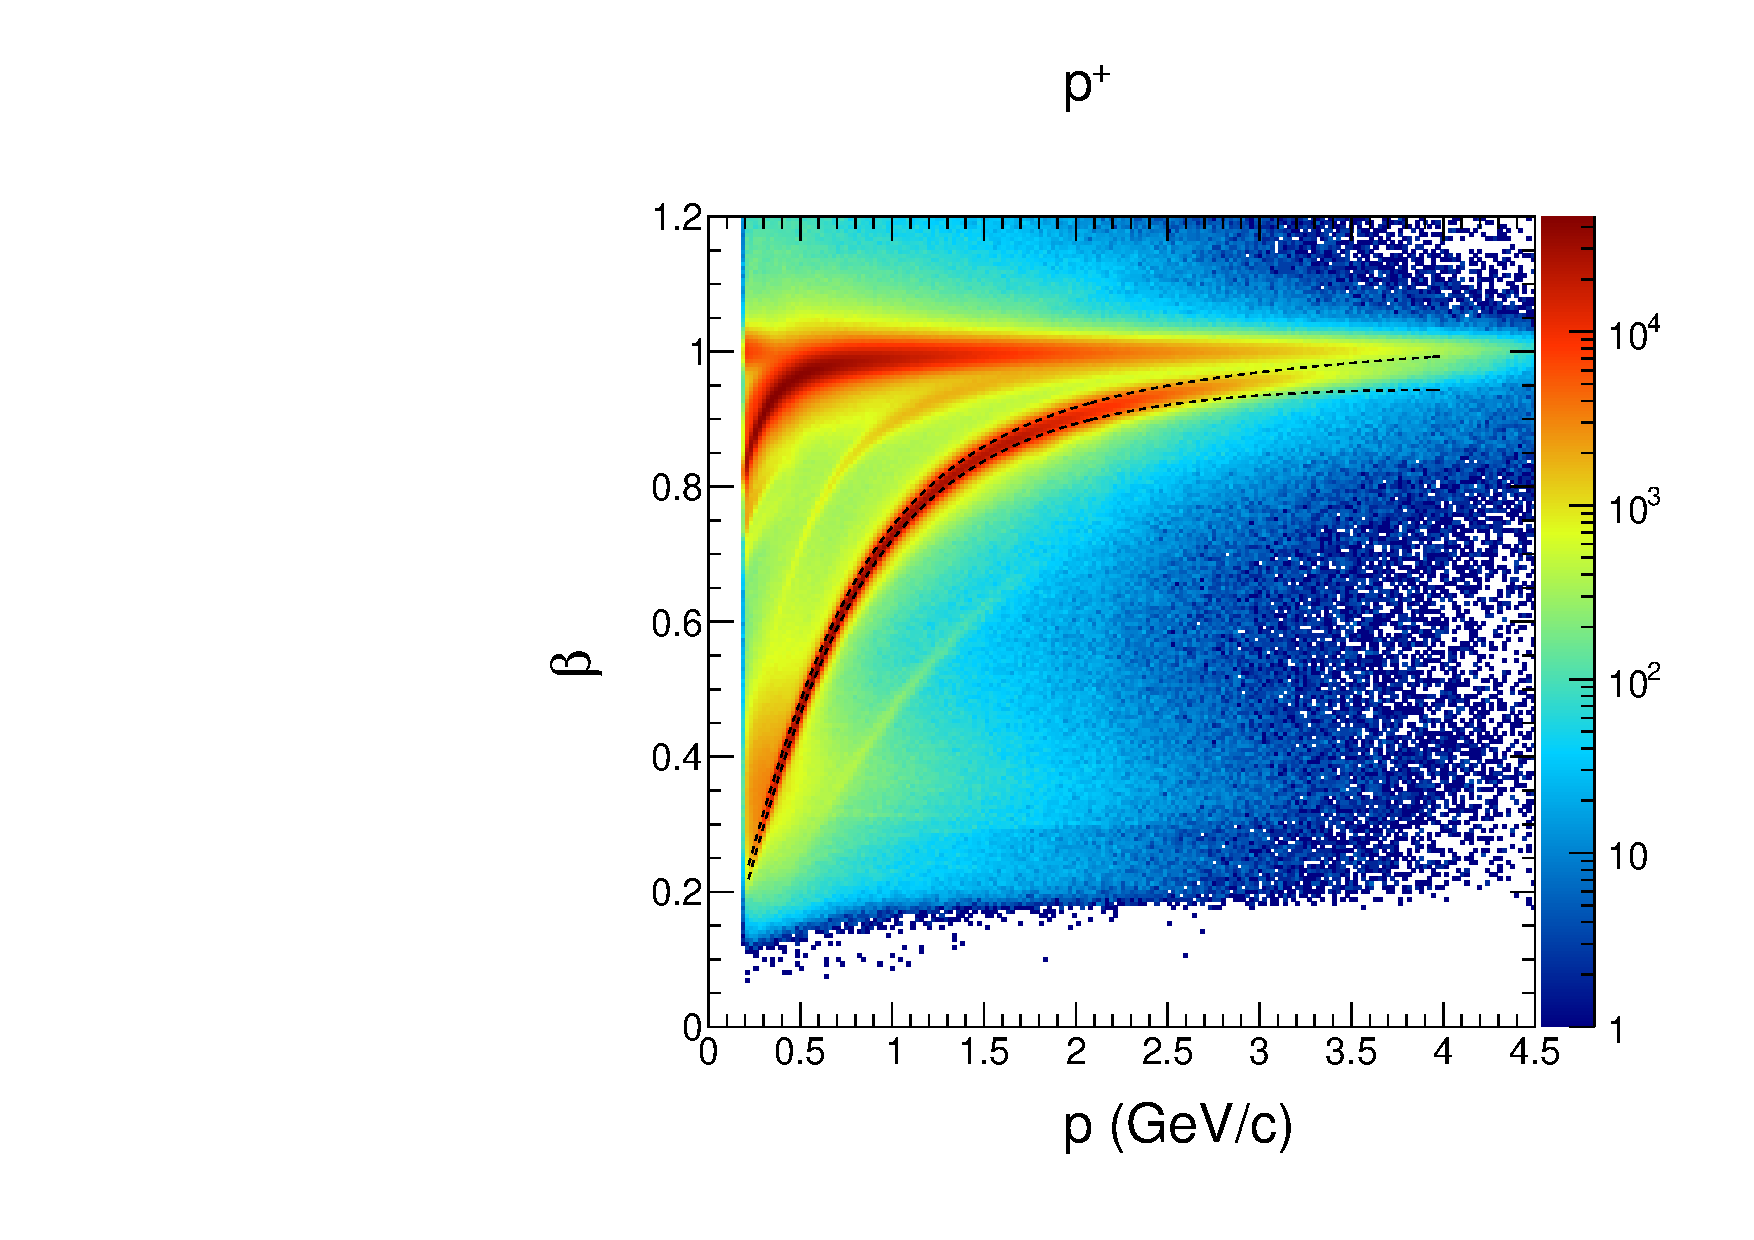
\includegraphics[width=10cm]{image/plots/hadron-id/beautiful_pbeta_prot.pdf}
    \caption{ Shown above: All positive tracks overlaid with our determination of $\mu(p) \pm \sigma(p)$ for $p^+$}
  \end{center}
\end{figure}

The parametrization used for the mean $\mu_ (p,h)$ and resolutions $\sigma (p,h)$ are shown below.

\begin{eqnarray}  
  \mu (p,h) = \mu_{theory} + \Delta \mu       \\
  \mu_{theory} = \frac{1}{\sqrt{1+(m_h/p)^2}} \\
  \Delta \mu = \mu_0 + \mu_1 p + \mu_2 p^2    \\
  \sigma (p,h) = \sigma_0 + \sigma_1 p + \sigma_2 p^2
\end{eqnarray}

The values are displayed in the table below. 

\begin{landscape}
  \begin{table}
%  \centering
  \begin{tabular}{c|c|c|c|c|c|c|c}
    Hadron & Parameter & Sector 1 & Sector 2 & Sector 3 & Sector 4 & Sector 5 & Sector 6 \\
    \hline 
      $K^+$ & $\mu_2$ & 0.00111554 & -8.97687e-05 &        4.78796e-05 &        0.000376425 &        -0.00204856 &        0.000652209 \\
       $K^+$ & $\mu_1$ & -0.00468038 & 6.19414e-05 &        -0.00081741 &       -0.00107931 &         0.00629181 &        -0.00264143 \\
       $K^+$ & $\mu_0$ & 0.00361012 &         0.00134921 &         0.00299674 &         0.00220194 &        0.000117821 &         0.00162582 \\
    $K^+$ & $\sigma_2$ & -0.000331838 &        -0.00105807 &       -0.000712404 &       -0.000573934 &       -0.000259289 &        0.000508389 \\
    $K^+$ & $\sigma_1$ & -0.00105857 &         0.00236686 &        0.000509169 &        0.000163467 &        -0.00233617 &        -0.00461598 \\
    $K^+$ & $\sigma_0$ & 0.0154964 &           0.0117702 &          0.0140748 &          0.0143761 &          0.0184055 &         0.0180945 \\
      $\pi^+$ & $\mu_2$ & -0.000962041 &       -0.000300602 &       -0.000306326 &        -3.2245e-05 &        -0.00226511 &       -0.000330818 \\
      $\pi^+$ & $\mu_1$ & 0.00296349 &          0.0016512 &          0.0021962 &         0.00176045 &         0.00750862 &         0.00126443 \\
      $\pi^+$ & $\mu_0$ & -0.00225794 &        -0.00047045 &        0.000370406 &        0.000435526 &       -0.000449409 &        -0.00131045 \\
   $\pi^+$ & $\sigma_2$ & -0.000127659 &        0.000691895 &       -0.000289961 &        0.000315041 &       -0.000936521 &       -0.000131269 \\
   $\pi^+$ & $\sigma_1$ & -0.000489092 &         -0.0033948 &         0.00196853 &       -0.00197841 &         0.00212778 &       -0.000339411 \\
   $\pi^+$ & $\sigma_0$ & 0.0155195 &           0.0167998 &          0.0124066 &          0.0157476 &          0.0145571 &         0.0141728 \\
     $p^+$ & $\mu_2$ & -0.00039358 &       -0.000701003 &       -0.000347651 &          0.0004854 &        -0.00121666  &       0.000563786 \\
     $p^+$ & $\mu_1$ & -0.000295423 &         0.00170899 &        0.000794901 &       -0.000744446 &         0.00376887 &        -0.00353545 \\
     $p^+$ & $\mu_0$ & 0.00227353 &         0.00231676 &         0.00364672 &         0.00276859 &         0.00128827 &          0.00439605 \\
  $p^+$ & $\sigma_2$ & 0.001429 &         0.00144256 &         0.00124456 &         0.00190709 &         0.00141039 &          0.0011516 \\
  $p^+$ & $\sigma_1$ & -0.0021472 &        -0.00262226 &        -0.00196308 &        -0.00385218 &        -0.00186708 &        -0.00186749 \\
  $p^+$ & $\sigma_0$ & 0.0107541 &          0.0109091 &          0.0104381 &          0.0115449 &          0.0109969 &          0.0107759 \\
      $\pi^-$ & $\mu_2$ & 3.28823666e-04 &    -1.30673670e-05 &    -2.32502052e-04 &    -9.75619848e-04 &    -5.89834444e-04 &     5.27496718e-04 \\
      $\pi^-$ & $\mu_1$ & -3.94924663e-03 &    -2.66028661e-03 &    -1.28565631e-03 &     9.09410075e-04 &    -2.01610684e-03 &    -4.42276918e-03 \\
      $\pi^-$ & $\mu_0$ & 9.48011169e-04 &     1.55078786e-03 &     1.43431985e-03 &     1.35056935e-03 &     4.59833580e-03 &     2.30751866e-03 \\
   $\pi^-$ & $\sigma_2$ & 4.37635504e-04 &     4.38306224e-04 &    5.32057510e-04 &     3.36999845e-04 &     7.74135462e-04 &     1.36515196e-04 \\
   $\pi^-$ & $\sigma_1$ & -3.28011836e-03 &    -3.28456104e-03 &    -3.82847286e-03 &     -3.11749323e-03 &    -4.63110728e-03 &    -2.21229710e-03 \\
   $\pi^-$ & $\sigma_0$ & 1.63296567e-02 &     1.62229164e-02 &    1.59769911e-02 &     1.58803427e-02 &     1.74670064e-02 &     1.51753145e-02 \\
       $K^-$ & $\mu_2$ & -2.72020947e-03 &    -5.21081786e-03 &    -2.13868763e-02 &    -4.45600034e-03 &    -7.60703841e-03 &    -5.27074813e-03 \\
       $K^-$ & $\mu_1$ & 1.78610401e-02 &      2.30787460e-02 &     9.49357818e-02 &     1.95764575e-02 &     3.63245785e-02 &     2.92417500e-02 \\
       $K^-$ & $\mu_0$ & -2.26190100e-02 &    -2.22562379e-02 &     -1.02704771e-01 &    -2.25931014e-02 &    -5.10484618e-02 &    -3.19918187e-02 \\
    $K^-$ & $\sigma_2$ & 1.76905114e-02 &     1.62989708e-02 &     3.60928130e-02 &     1.51270521e-02 &     1.91308107e-02 &     2.38470033e-02 \\
    $K^-$ & $\sigma_1$ & -7.74901862e-02 &    -7.33041628e-02 &    -1.57454534e-01 &    -7.26870393e-02 &     -9.23654247e-02 &    -1.02397836e-01 \\
    $K^-$ & $\sigma_0$ & 1.07082820e-01 &     1.00573410e-01 &     1.93148260e-01 &     1.00993689e-01 &     1.26963814e-01 &     1.30057621e-01
  \end{tabular}
  \caption{Values used to calculate the mean and resolutions for hadron likelihood based identification.}
  \label{table-hadron-pdfs}
  \end{table}
\end{landscape}




